% Substituição da Nota Editorial 2 — Estudos de Caso Reais Mascarados e Reconciliação
\begin{figure}[htbp]
  \centering
  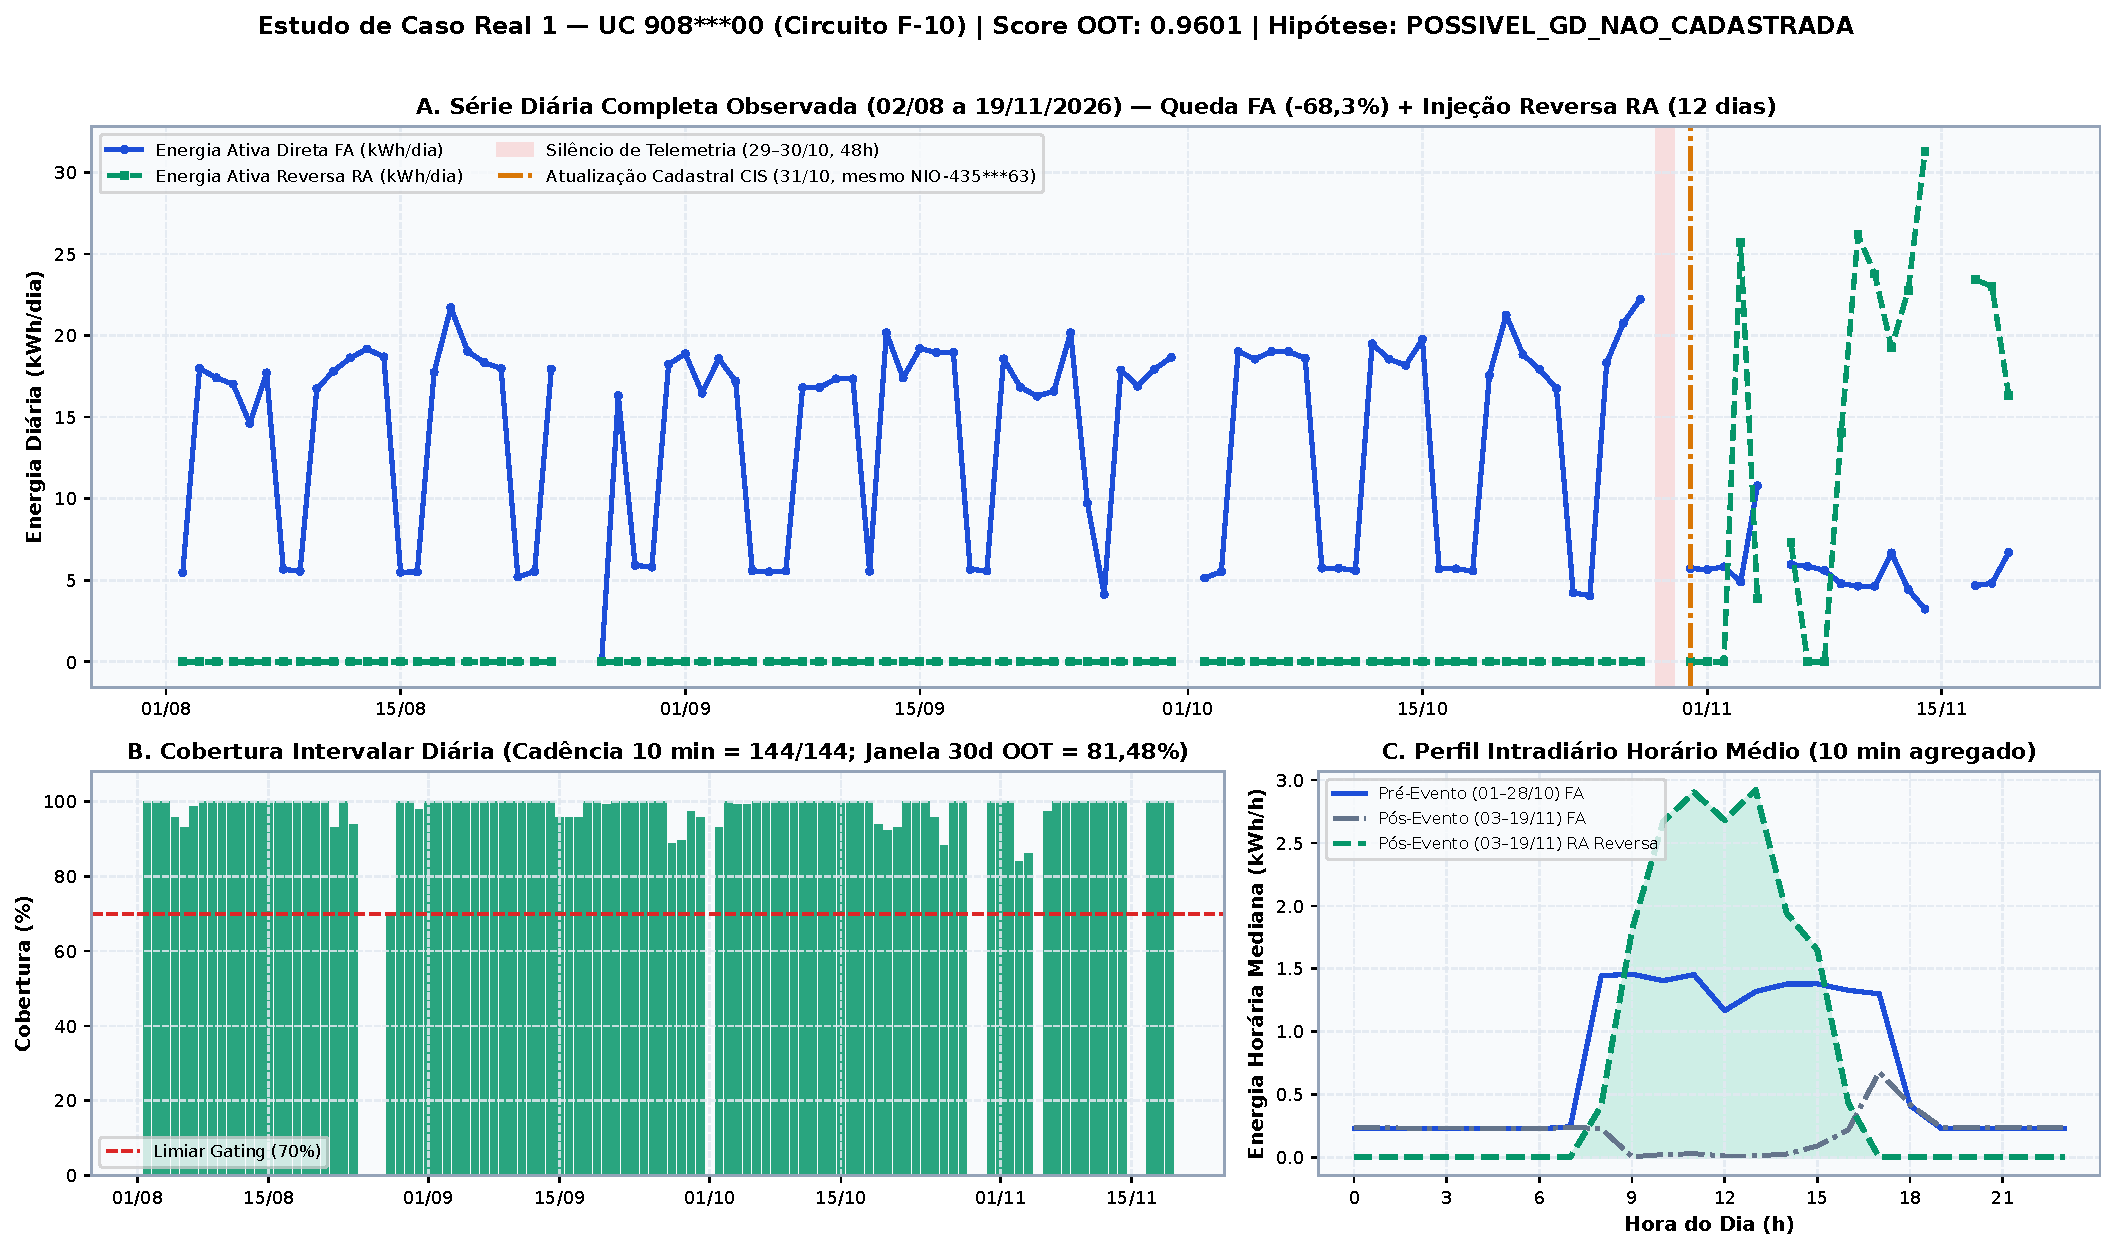
\includegraphics[width=0.98\textwidth]{manuscript_figures/real_case_studies/fig_caso_908xxx00_fa_ra_completo.pdf}
  \caption{Série temporal completa observada para a UC \texttt{908***00} (02/08 a 19/11/2026, medidor \texttt{NIO-435***63}, \texttt{run\_id = 20261123\_124416\_146\_oot\_multiview}): (A) energia ativa direta FA e reversa RA diárias; (B) cobertura ajustada à cadência de 10~min; (C) perfis horários médios pré e pós-31/10.}
  \label{fig:caso-908xxx00-completo}
\end{figure}

\begin{figure}[htbp]
  \centering
  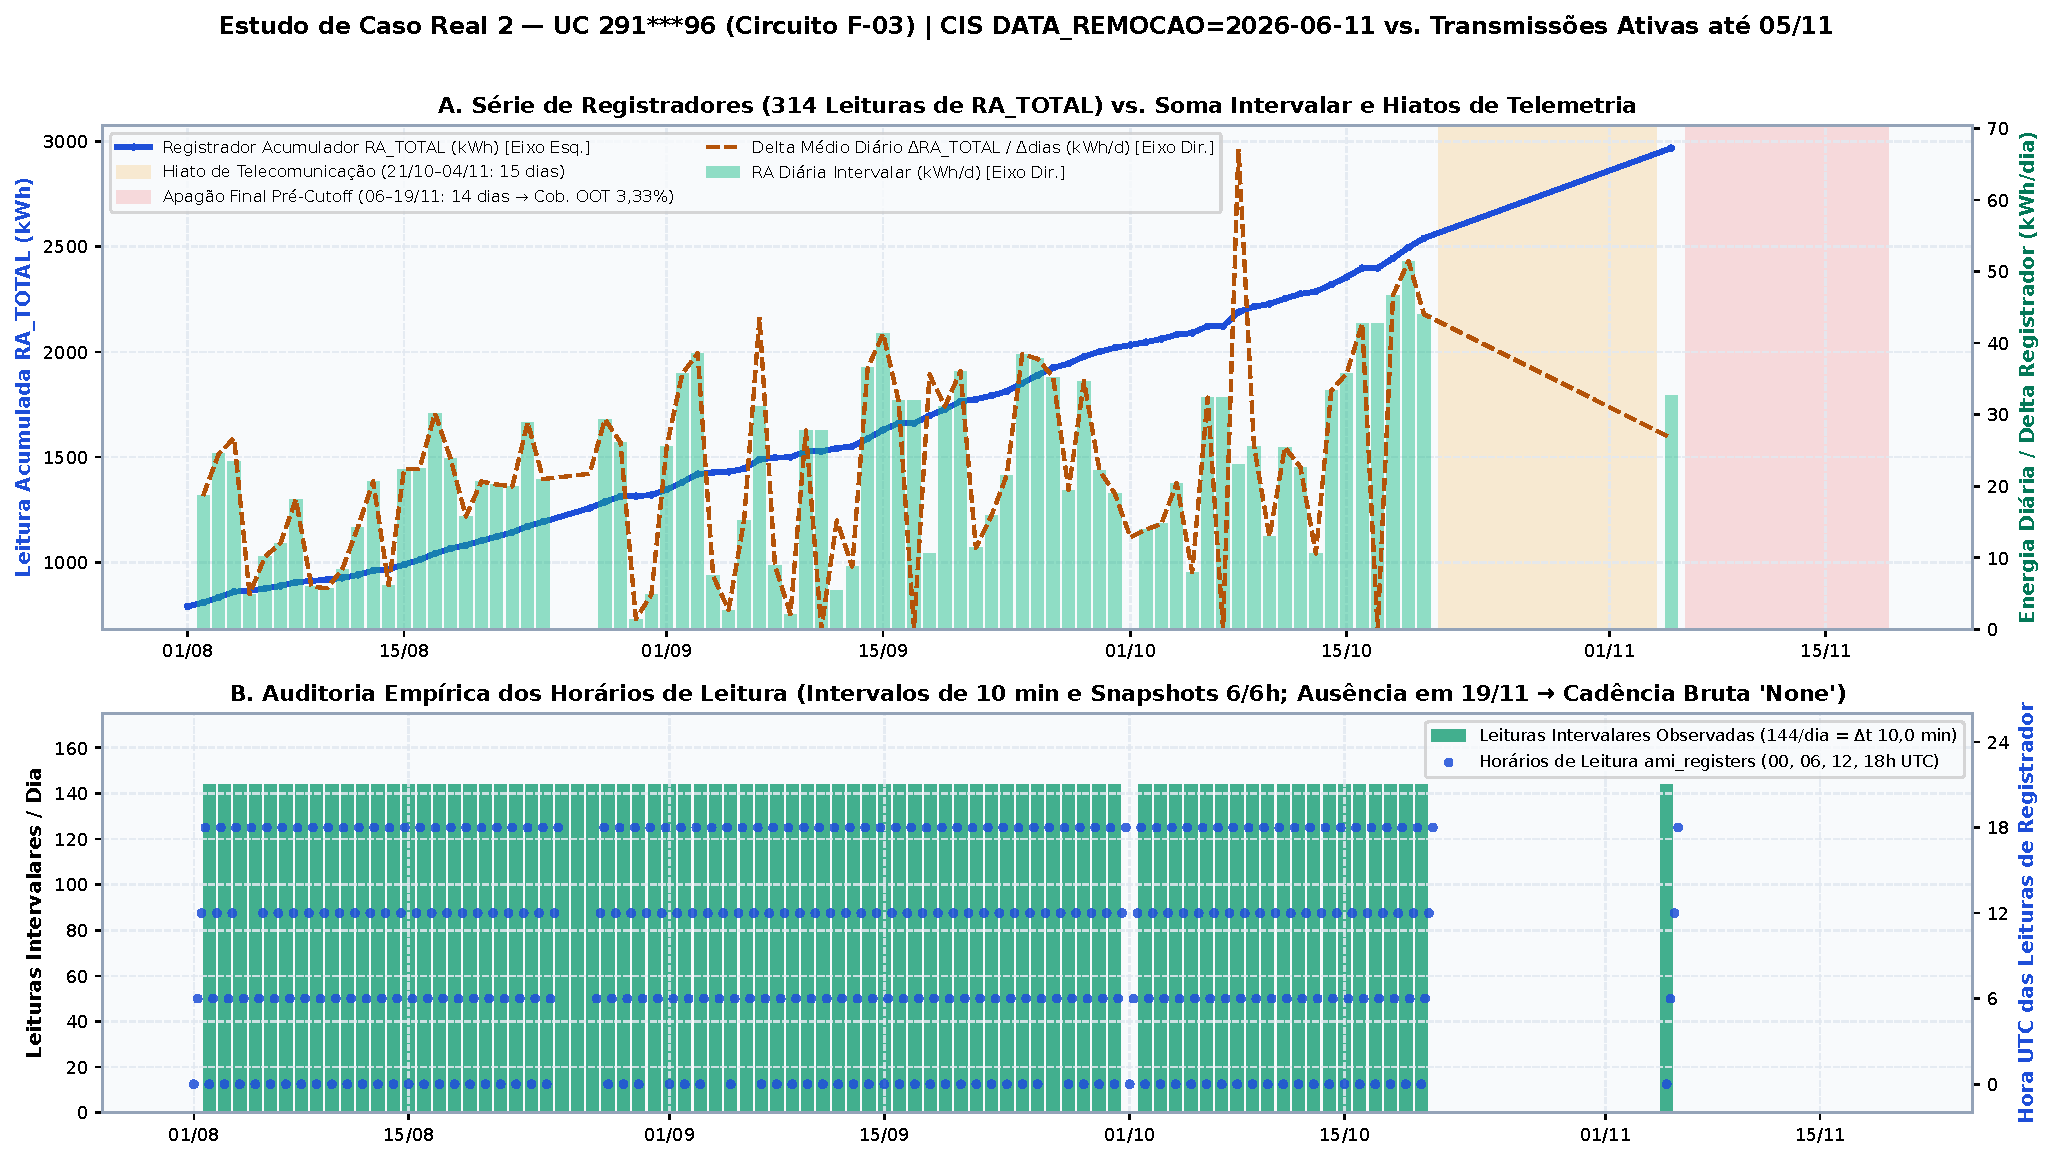
\includegraphics[width=0.98\textwidth]{manuscript_figures/real_case_studies/fig_caso_291xxx96_horarios_registradores.pdf}
  \caption{Auditoria longitudinal da UC \texttt{291***96} (\texttt{NIO-423***54}, 01/08 a 19/11/2026): (A) evolução acumulada de 314 leituras do registrador \texttt{RA\_TOTAL} ($764{,}601 \to 2.967{,}725$~kWh), delta diário e hiatos de comunicação; (B) horários empíricos de leitura intervalar (10~min) e de registradores (00h/06h/12h/18h UTC).}
  \label{fig:caso-291xxx96-registradores}
\end{figure}

\begin{figure}[htbp]
  \centering
  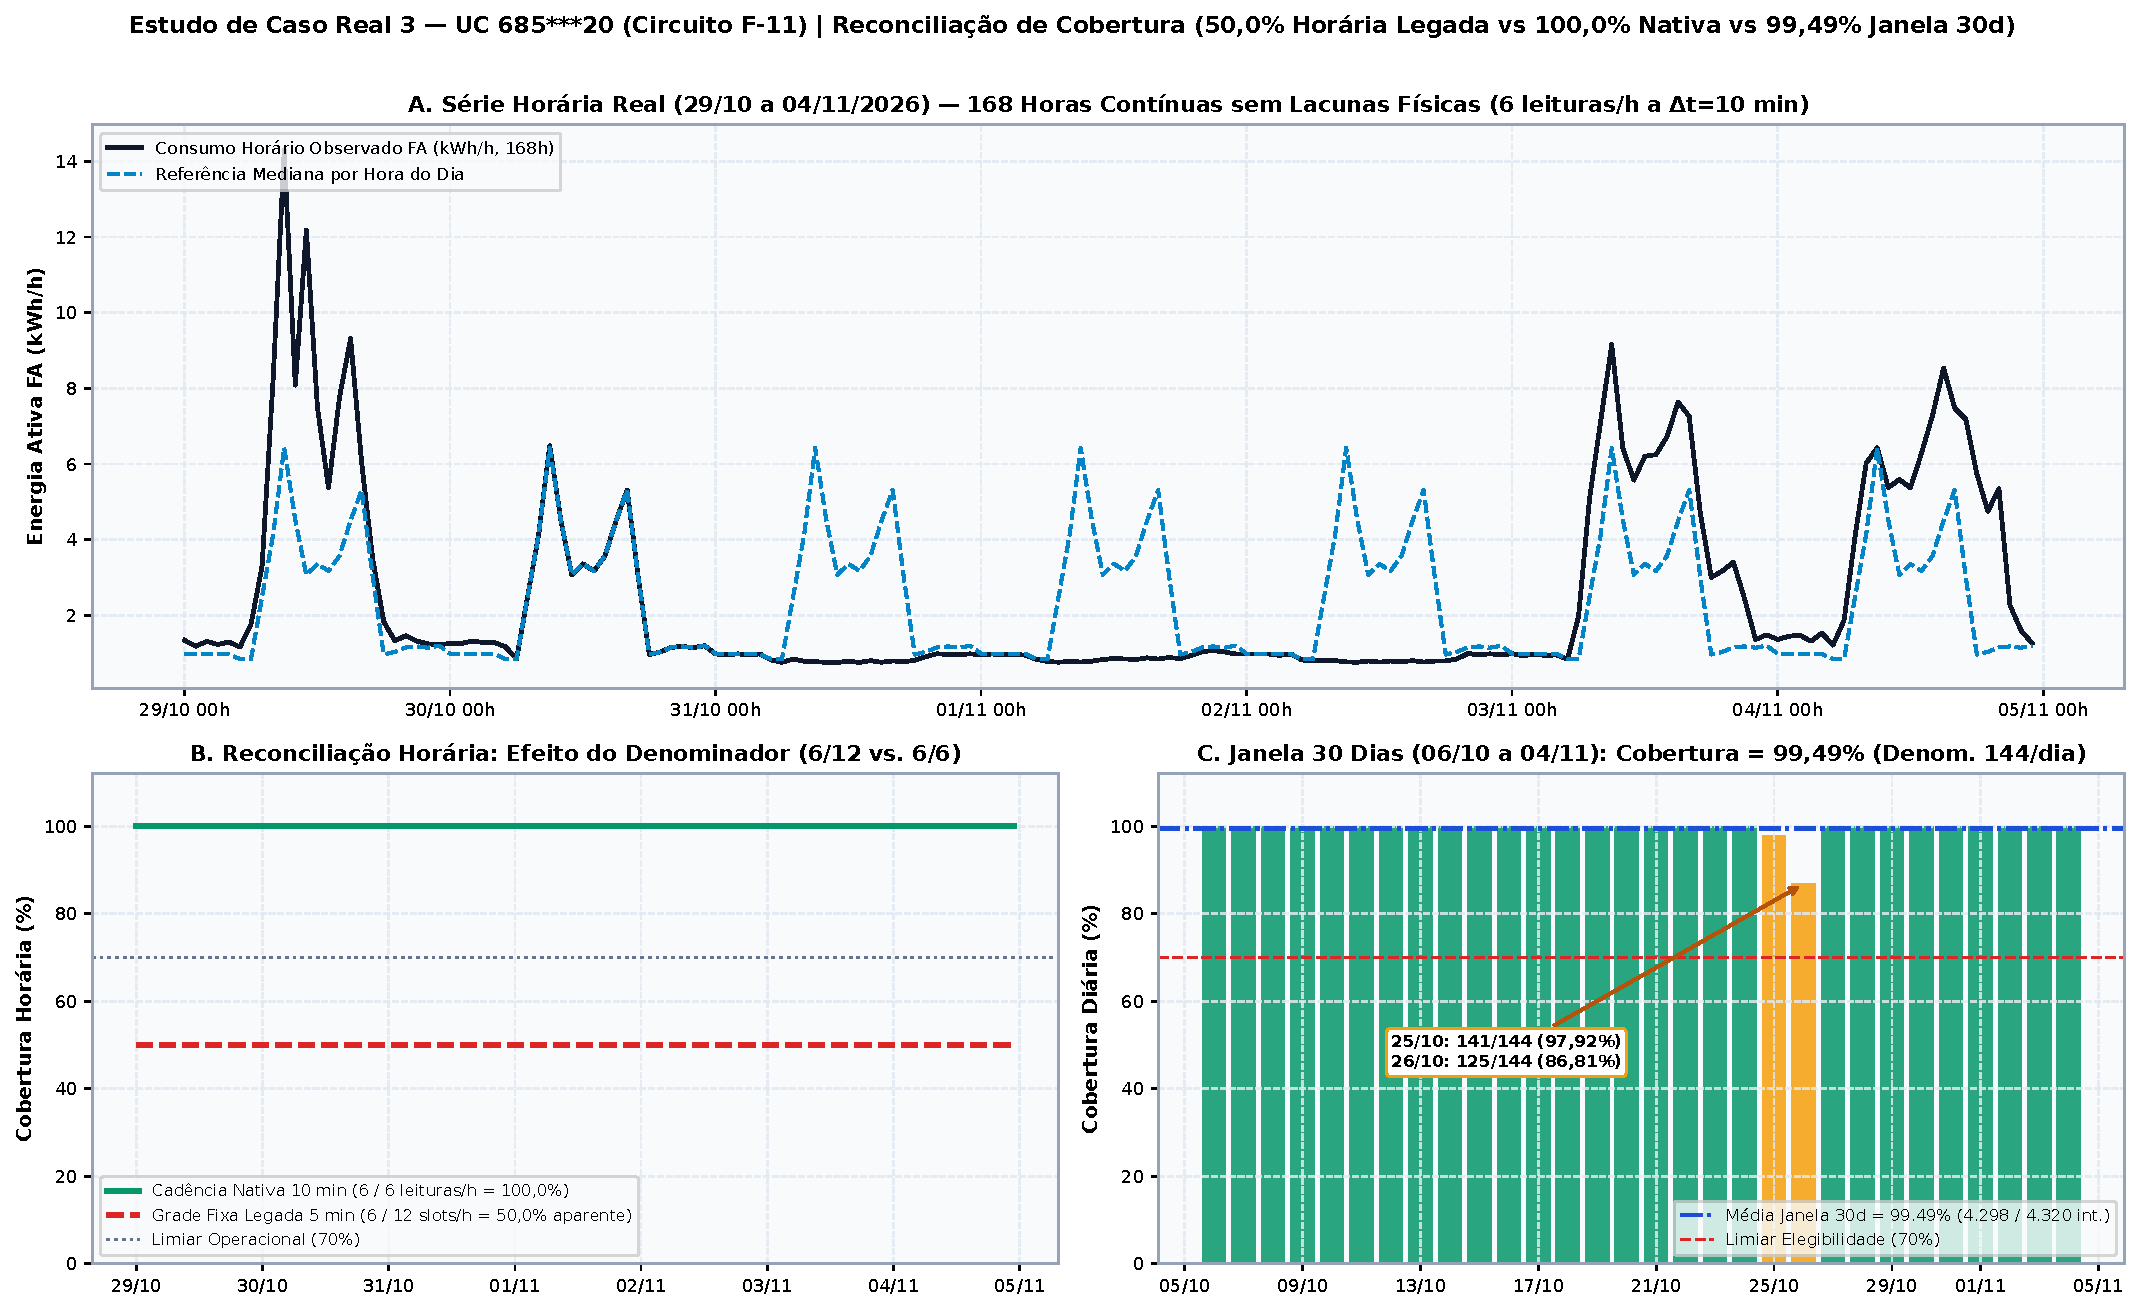
\includegraphics[width=0.98\textwidth]{manuscript_figures/real_case_studies/fig_caso_685xxx20_reconciliacao_cobertura.pdf}
  \caption{Reconciliação da cobertura da UC \texttt{685***20} (\texttt{NIO-437***86}, cadência nativa $\Delta t = 10$~min): (A) série horária observada (168h entre 29/10 e 04/11/2026); (B) cobertura horária em grade fixa de 5~min ($6/12 = 50{,}0\%$) versus cadência nativa de 10~min ($6/6 = 100{,}0\%$); (C) janela de 30 dias em \texttt{uc\_day\_features} ($4.298 / 4.320 = 99{,}49\%$).}
  \label{fig:caso-685xxx20-reconciliacao}
\end{figure}

\begin{table}[htbp]
  \centering
  \caption{Reconciliação formal entre representações de cobertura observadas para a UC \texttt{685***20} (\texttt{NIO-437***86}) sem alteração de valores originais.}
  \label{tab:reconciliacao-uc-685xxx20}
  \small
  \begin{tabular}{llllrrl}
    \toprule
    \textbf{Representação} & \textbf{Canal} & \textbf{Cadência} & \textbf{Período} & \textbf{Numerador} & \textbf{Denominador} & \textbf{Valor} \\
    \midrule
    Horária (grade legada) & \texttt{ami\_interval.FA} & 10~min & 168h (29/10--04/11) & 6 leit./h & 12 slots/h (5~min) & 50,00\% \\
    Horária (ajustada) & \texttt{ami\_interval.FA} & 10~min & 168h (29/10--04/11) & 6 leit./h & 6 slots/h (10~min) & 100,00\% \\
    Janela 30 dias & \texttt{uc\_day\_features} & 10~min & 30d (06/10--04/11) & 4.298 int. & 4.320 ($30\times 144$) & 99,49\% \\
    Instantânea diária & \texttt{ami\_instantaneous} & 20~min & Diário (30d) & 72 leit./d & 288 slots/d & 25,00\% \\
    \bottomrule
  \end{tabular}
\end{table}

Os três casos reais anonimizados ilustram a resolução diferencial sem afirmação causal prematura. Na Figura~\ref{fig:caso-908xxx00-completo}, a UC~\texttt{908***00} mantém o mesmo medidor após atualização cadastral em 31/10/2026 e passa a apresentar retração de consumo direto associada a 12 dias de fluxo reverso ativo. Na Figura~\ref{fig:caso-291xxx96-registradores}, embora o cadastro comercial aponte remoção anterior e o período final (06--19/11) apresente silêncio completo (cadência pontual \texttt{None} em 19/11 e cobertura de 3,33\% na janela OOT), as 314 leituras anteriores confirmam integração física contínua do registrador até 05/11, justificando a retenção na fila técnica de telecomunicação. Por fim, a Figura~\ref{fig:caso-685xxx20-reconciliacao} e a Tabela~\ref{tab:reconciliacao-uc-685xxx20} demonstram que os valores 50,0\% e 99,49\% da UC~\texttt{685***20} coexistem de forma matematicamente consistente ao distinguir canal, cadência nativa (10~min), período e denominador adotado.
